\documentclass[tikz,border=2pt]{standalone}
\usepackage{amsmath}
\usepackage{tikz}
\usetikzlibrary{arrows.meta}

\begin{document}
% A function sends every input to exactly one output. Left: a function (two inputs may share an
% output). Right: not a function, because one input has two arrows.
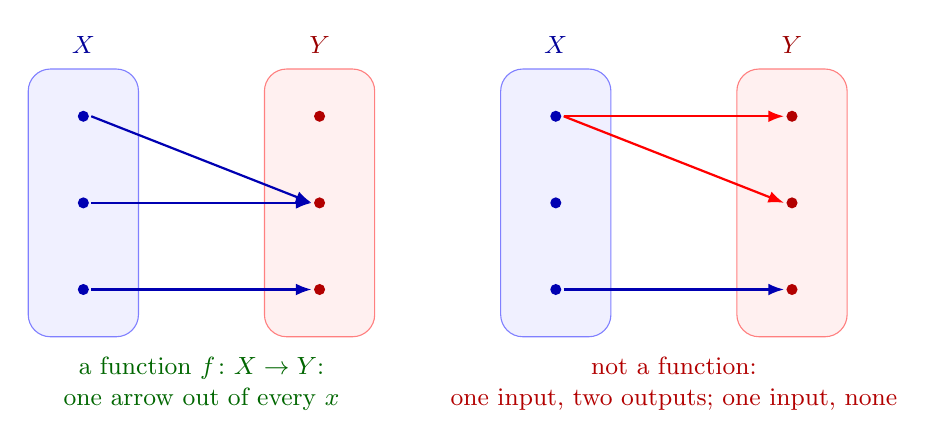
\begin{tikzpicture}[>={Latex[length=2mm]}, every node/.style={font=\small}]
	\begin{scope}
		\draw[rounded corners=8pt, fill=blue!6, draw=blue!50] (-0.7,-1.7) rectangle (0.7,1.7);
		\draw[rounded corners=8pt, fill=red!6, draw=red!50] (2.3,-1.7) rectangle (3.7,1.7);
		\node[blue!60!black] at (0,2.0) {$X$}; \node[red!60!black] at (3,2.0) {$Y$};
		\foreach \y in {1.1,0,-1.1} {\fill[blue!70!black] (0,\y) circle (2pt);}
		\foreach \y in {1.1,0,-1.1} {\fill[red!70!black] (3,\y) circle (2pt);}
		\draw[->, blue!70!black, thick] (0.1,1.1) -- (2.9,0);
		\draw[->, blue!70!black, thick] (0.1,0) -- (2.9,0);
		\draw[->, blue!70!black, thick] (0.1,-1.1) -- (2.9,-1.1);
		\node[green!40!black, align=center] at (1.5,-2.3) {a function $f\colon X\to Y$:\\ one arrow out of every $x$};
	\end{scope}
	\begin{scope}[xshift=6cm]
		\draw[rounded corners=8pt, fill=blue!6, draw=blue!50] (-0.7,-1.7) rectangle (0.7,1.7);
		\draw[rounded corners=8pt, fill=red!6, draw=red!50] (2.3,-1.7) rectangle (3.7,1.7);
		\node[blue!60!black] at (0,2.0) {$X$}; \node[red!60!black] at (3,2.0) {$Y$};
		\foreach \y in {1.1,0,-1.1} {\fill[blue!70!black] (0,\y) circle (2pt);}
		\foreach \y in {1.1,0,-1.1} {\fill[red!70!black] (3,\y) circle (2pt);}
		\draw[->, red, thick] (0.1,1.1) -- (2.9,1.1);
		\draw[->, red, thick] (0.1,1.1) -- (2.9,0);
		\draw[->, blue!70!black, thick] (0.1,-1.1) -- (2.9,-1.1);
		\node[red!70!black, align=center] at (1.5,-2.3) {not a function:\\ one input, two outputs; one input, none};
	\end{scope}
\end{tikzpicture}
\end{document}
